\block{}{\centering
  \begin{tikzfigure}%[First iteration of Phase 1]
    %
    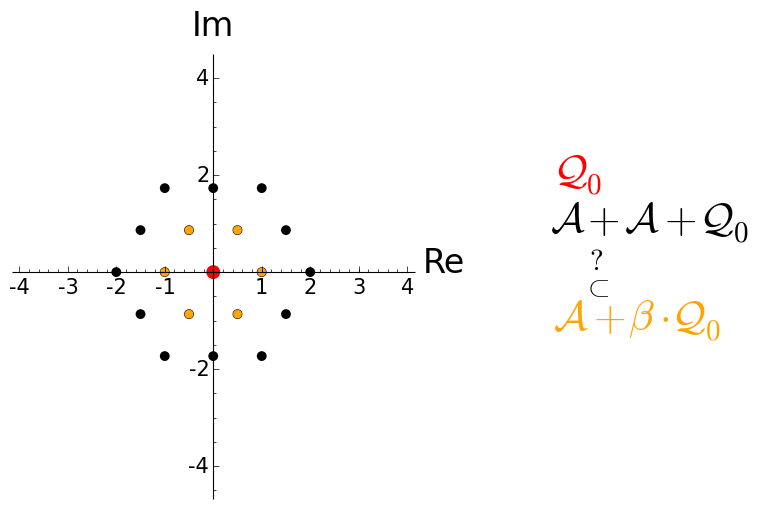
\includegraphics[width=0.2\textwidth]{img/phase1_image_3a.png}
    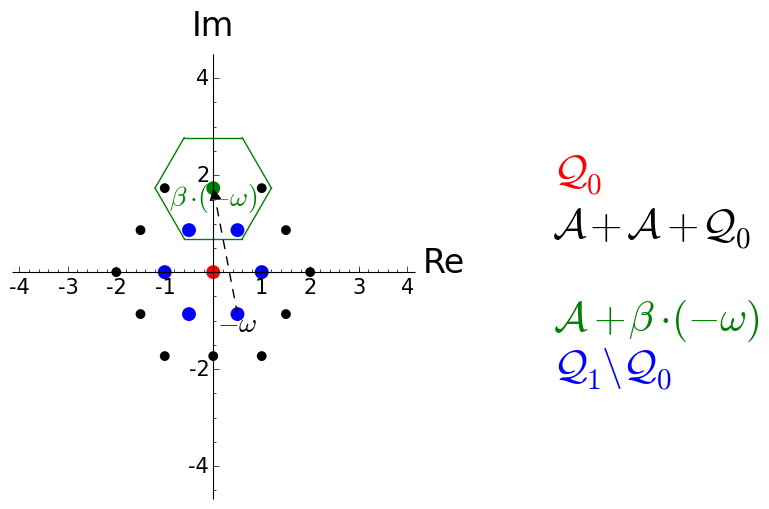
\includegraphics[width=0.2\textwidth]{img/phase1_image_4.png}
\end{tikzfigure}
First iteration of Phase 1
\vspace{13pt}
}

\note[targetoffsetx=-.21\colwidth,targetoffsety=-0.105\colwidth,innersep=0.5cm,angle=-135, width=.55\subcolwidth]{Figures are plotted for Eisenstein base $$\beta = \omega -1\,,\omega=\imath\,\frac{1}{2} \sqrt{3}-\frac{1}{2}$$
%
%with the minimal polynomial $$m_\beta(x)=x^2+3x+3\,.$$
% 
and the alphabet $$\mathcal{A} =\{0, 1, -1, \omega, -\omega, -\omega - 1, \omega + 1\}$$}
